% 图 8.1 (a) 正方晶格上的反铁磁完全排布 (b) 三角晶格上的几何阻挫（第三自旋无法满足）
\documentclass[tikz,border=5pt]{standalone}
\usetikzlibrary{arrows.meta,calc}
\usepackage{amsmath}
\usepackage{bm}
\usepackage{fontspec}
\setmainfont{Times New Roman}
\begin{document}
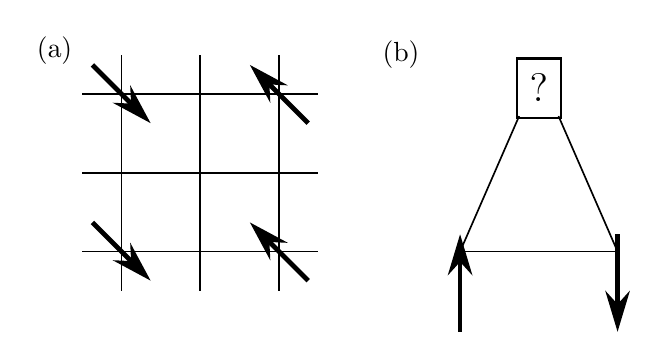
\begin{tikzpicture}[line width=0.8pt,>=Stealth]
\tikzset{spinstick/.style={line width=1.7pt,-{Stealth[length=5.2mm,width=3.1mm]}}}
% ---------- (a) square lattice, 2x2 cells, AFM spins on corners ----------
\begin{scope}[shift={(0,0)}]
  \draw[line width=0.6] (-0.5,0) -- (2.5,0);
  \draw[line width=0.6] (-0.5,1) -- (2.5,1);
  \draw[line width=0.6] (-0.5,2) -- (2.5,2);
  \draw[line width=0.6] (0,-0.5) -- (0,2.5);
  \draw[line width=0.6] (1,-0.5) -- (1,2.5);
  \draw[line width=0.6] (2,-0.5) -- (2,2.5);
  % spins on the four corners: diagonal matchsticks, adjacent antiparallel
  \draw[spinstick] ($(0,2)+(-0.37,0.37)$)  -- ($(0,2)+(0.37,-0.37)$);   % TL: SE
  \draw[spinstick] ($(2,2)+(0.37,-0.37)$)  -- ($(2,2)+(-0.37,0.37)$);   % TR: NW
  \draw[spinstick] ($(0,0)+(-0.37,0.37)$)  -- ($(0,0)+(0.37,-0.37)$);   % BL: SE
  \draw[spinstick] ($(2,0)+(0.37,-0.37)$)  -- ($(2,0)+(-0.37,0.37)$);   % BR: NW
  \node at (-0.85,2.55) {(a)};
\end{scope}
% ---------- (b) triangular cell: two spins antiparallel, third frustrated ----------
\begin{scope}[shift={(4.3,0)}]
  \draw[line width=0.6] (0,0) -- (2,0);                       % base
  \draw[line width=0.6] (0.75,1.72) -- (0,0);                 % left side (from box)
  \draw[line width=0.6] (1.25,1.72) -- (2,0);                 % right side (from box)
  \draw[line width=0.8] (0.72,1.70) rectangle (1.28,2.45);    % box at apex
  \node at (1,2.075) {\Large ?};
  \draw[spinstick] (0,-1.02) -- (0,0.22);                     % left spin: up
  \draw[spinstick] (2,0.22) -- (2,-1.02);                     % right spin: down
  \node at (-0.75,2.5) {(b)};
\end{scope}
\end{tikzpicture}
\end{document}
